\section{Mätinstrument}

\subsection{Presentation av mätvärden}

\begin{wrapfigure}[20]{R}{0.5\textwidth}
  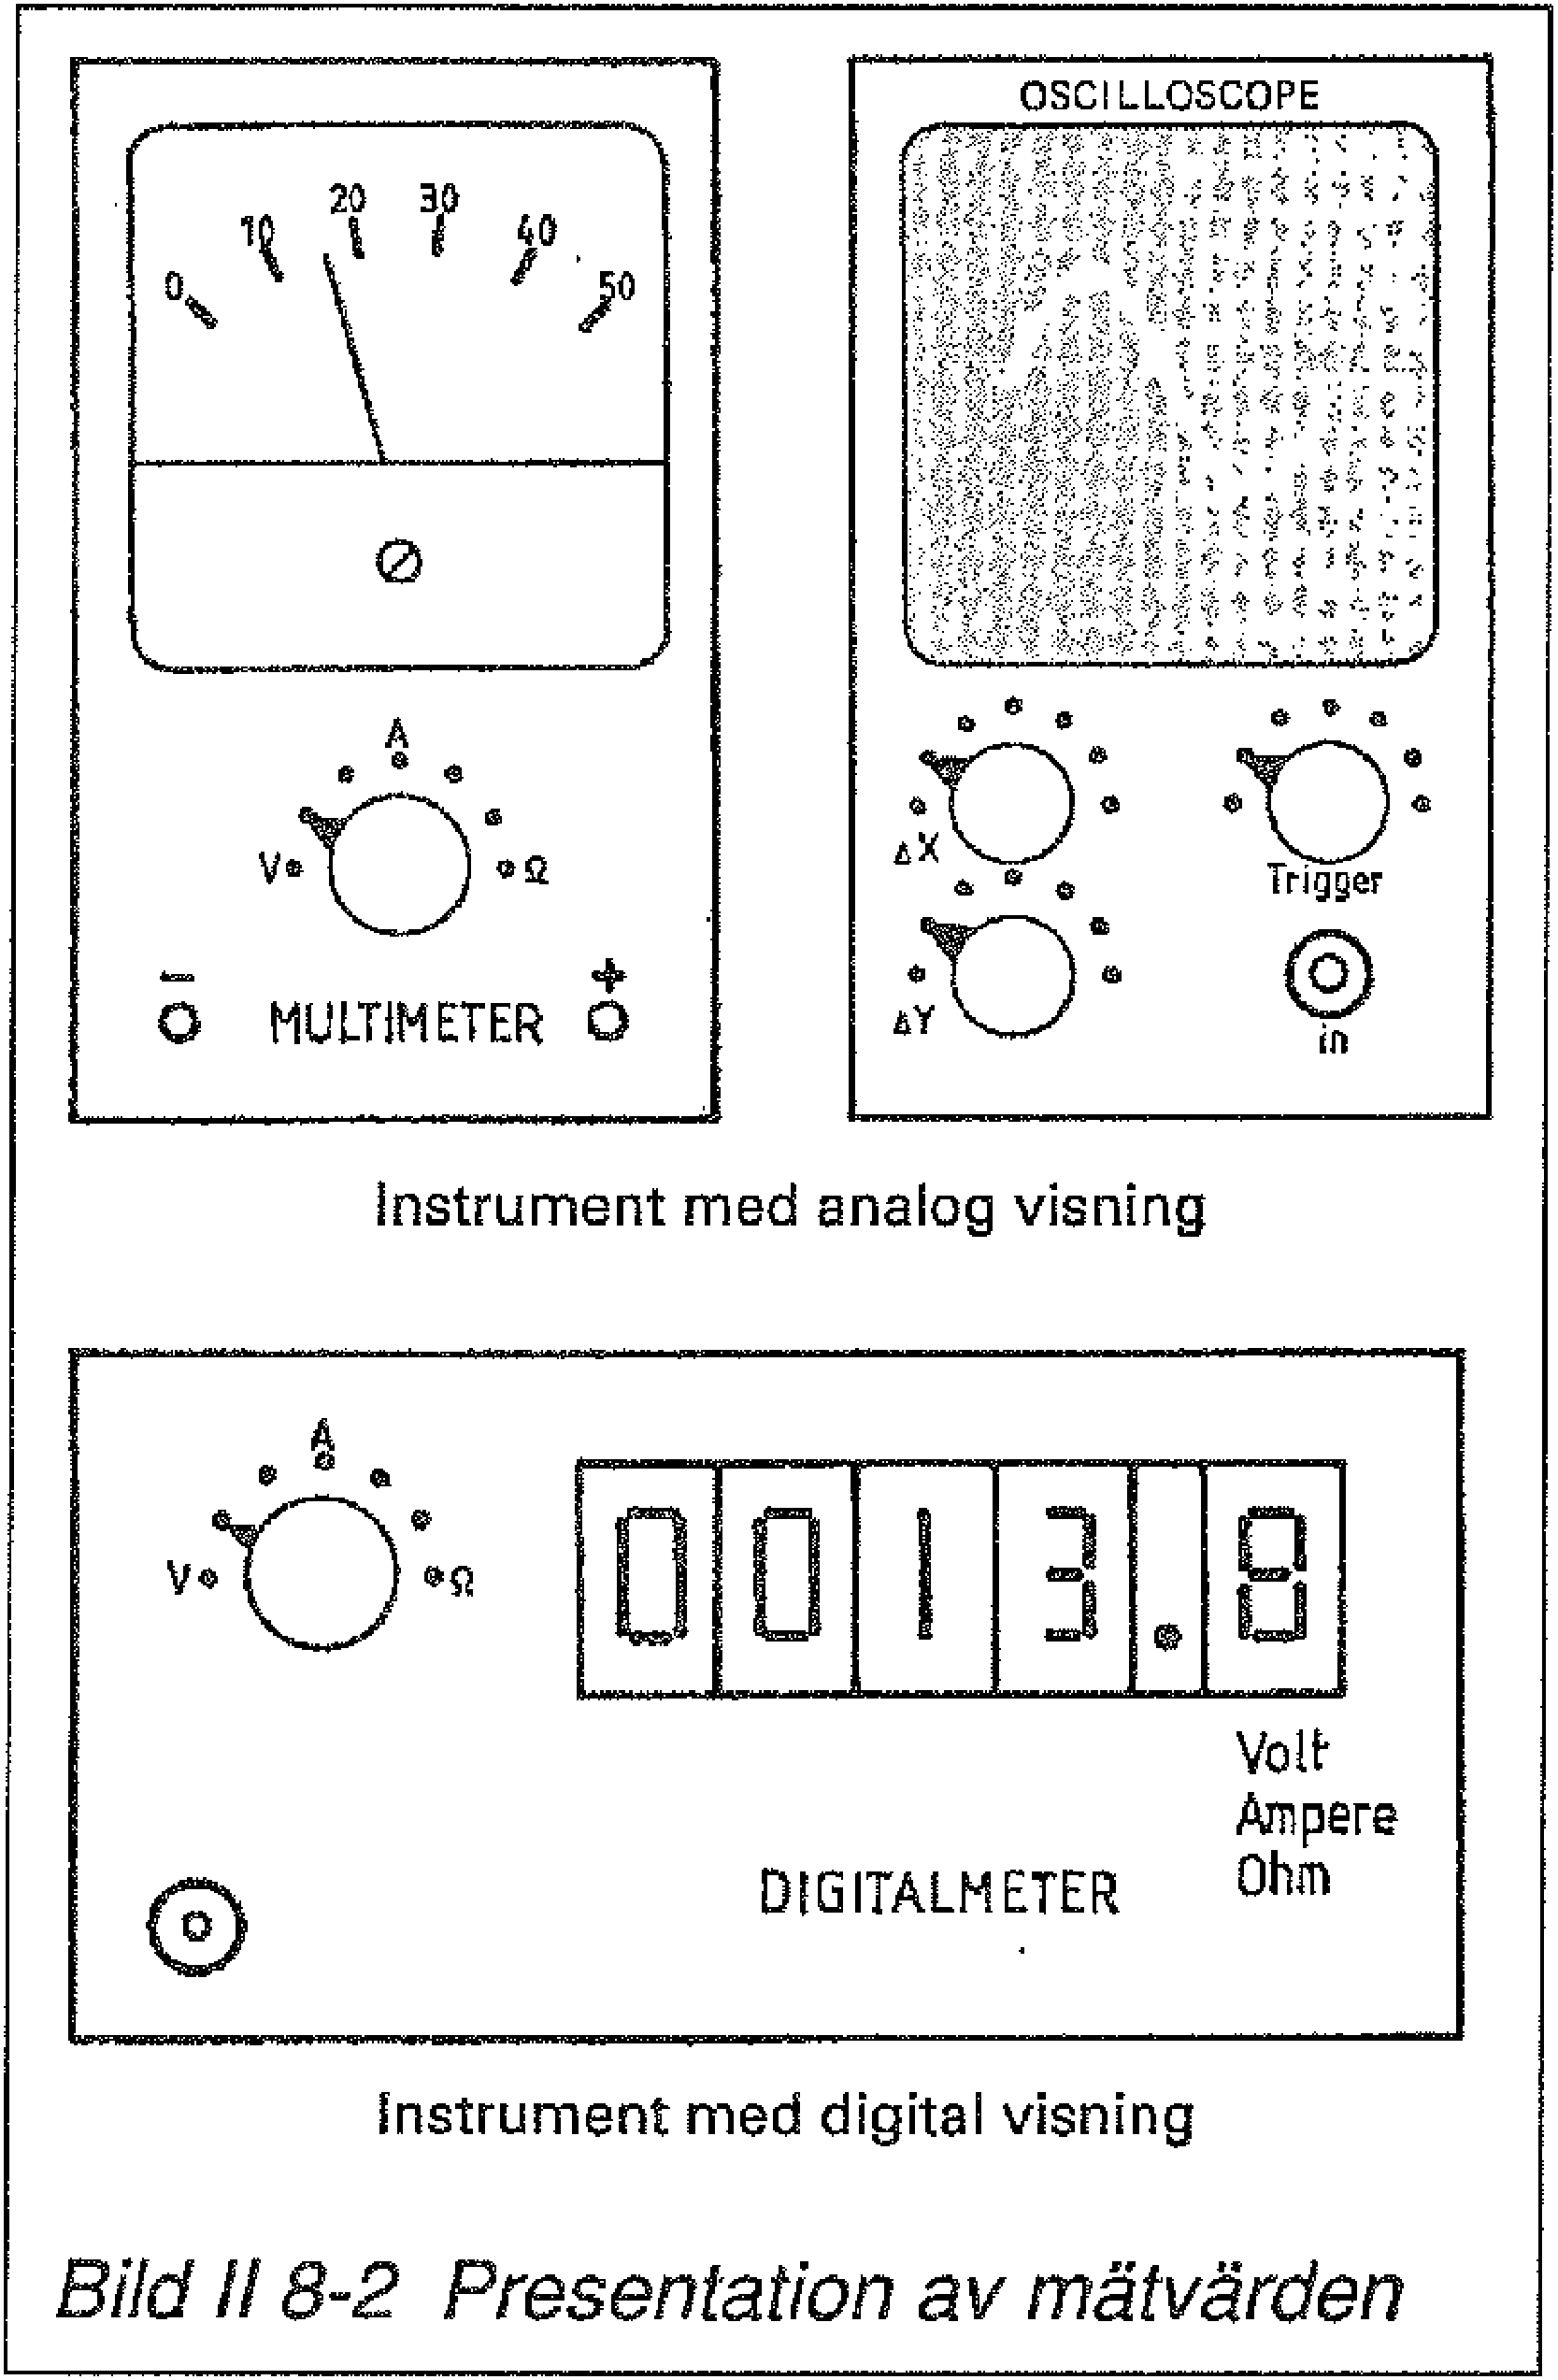
\includegraphics[width=0.5\textwidth]{images/bild_2_8-02}
  \caption{Presentation av mätvärden}
  \label{fig:bildII8-2}
\end{wrapfigure}

Bild \ref{fig:bildII8-2}

Mätvärden kan presenteras på olika sätt. De vanligaste sätten är
optiska och då med digital eller analog visning. Mätresultat kan även
överföras till dator för vidare bearbetning och visning.

\subsection{Multimeter}
\textbf{
HAREC a.\ref{HAREC.a.8.2.1.1}\label{myHAREC.a.8.2.1.1}
}

Bild \ref{fig:bildII8-2}

Flera mätfunktioner kan utföras med samma basinstrument. Genom
omkoppling mellan olika tillsatser väljer man mätfunktion och
mätområde. Instrumentskalan utformas så att olika slags mätvärden kan
avläsas.  Kombinationer med elektroniska förstärkare och digital
visning etc. är nu vanligt.

\subsection{Vridspoleinstrument}

\begin{figure}
  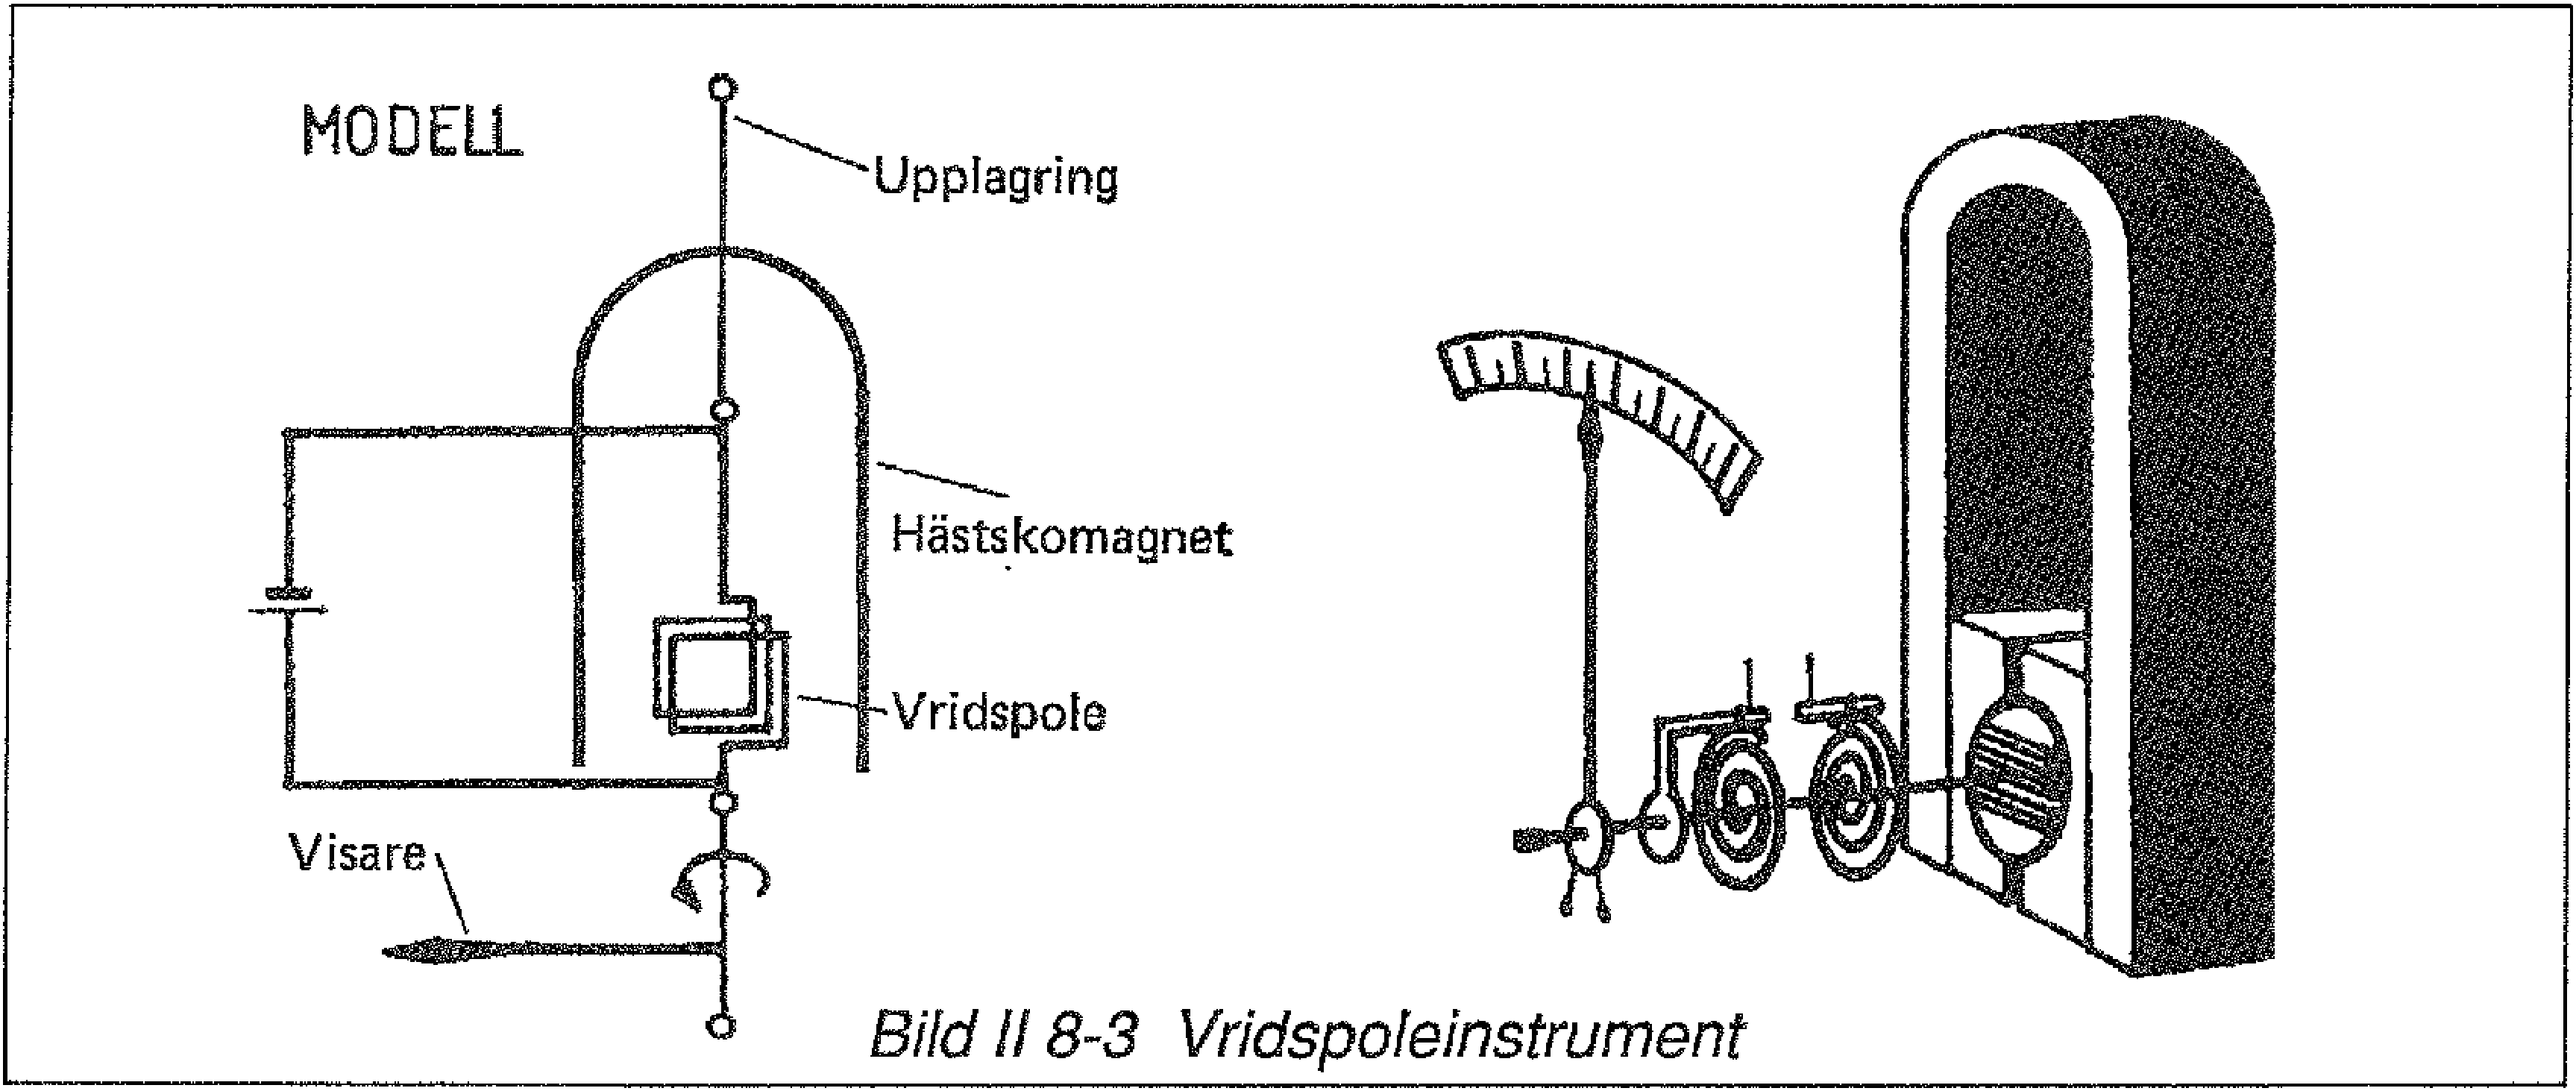
\includegraphics[width=\textwidth]{images/bild_2_8-03}
  \caption{Vridspoleinstrument}
  \label{fig:bildII8-3}
\end{figure}

Bild \ref{fig:bildII8-3}

Vridspoleinstrument kan bara användas för likströmsmätning, eftersom
visarutslaget beror av strömriktningen. Instrumentet har låg
effektförbrukning och stor noggrannhet.  Visningen är vanligen linjär,
men kan göras annorlunda.

Funktion: En spole är upplagrad i fältet av en hästskomagnet När den
ström, som ska mätas, passerar genom den vridbara spolen så alstras
ett magnetfält även i denna. De två magnetfälten påverkarvarandra så
att spolen vrider sig. Spolen förses med en visare och en
returfjäder. Ju större ström det flyter genom spolen desto större blir
visarutslaget

\begin{rev-raderas}
\subsection{Mjukjärnsinstrument}

\begin{figure}
  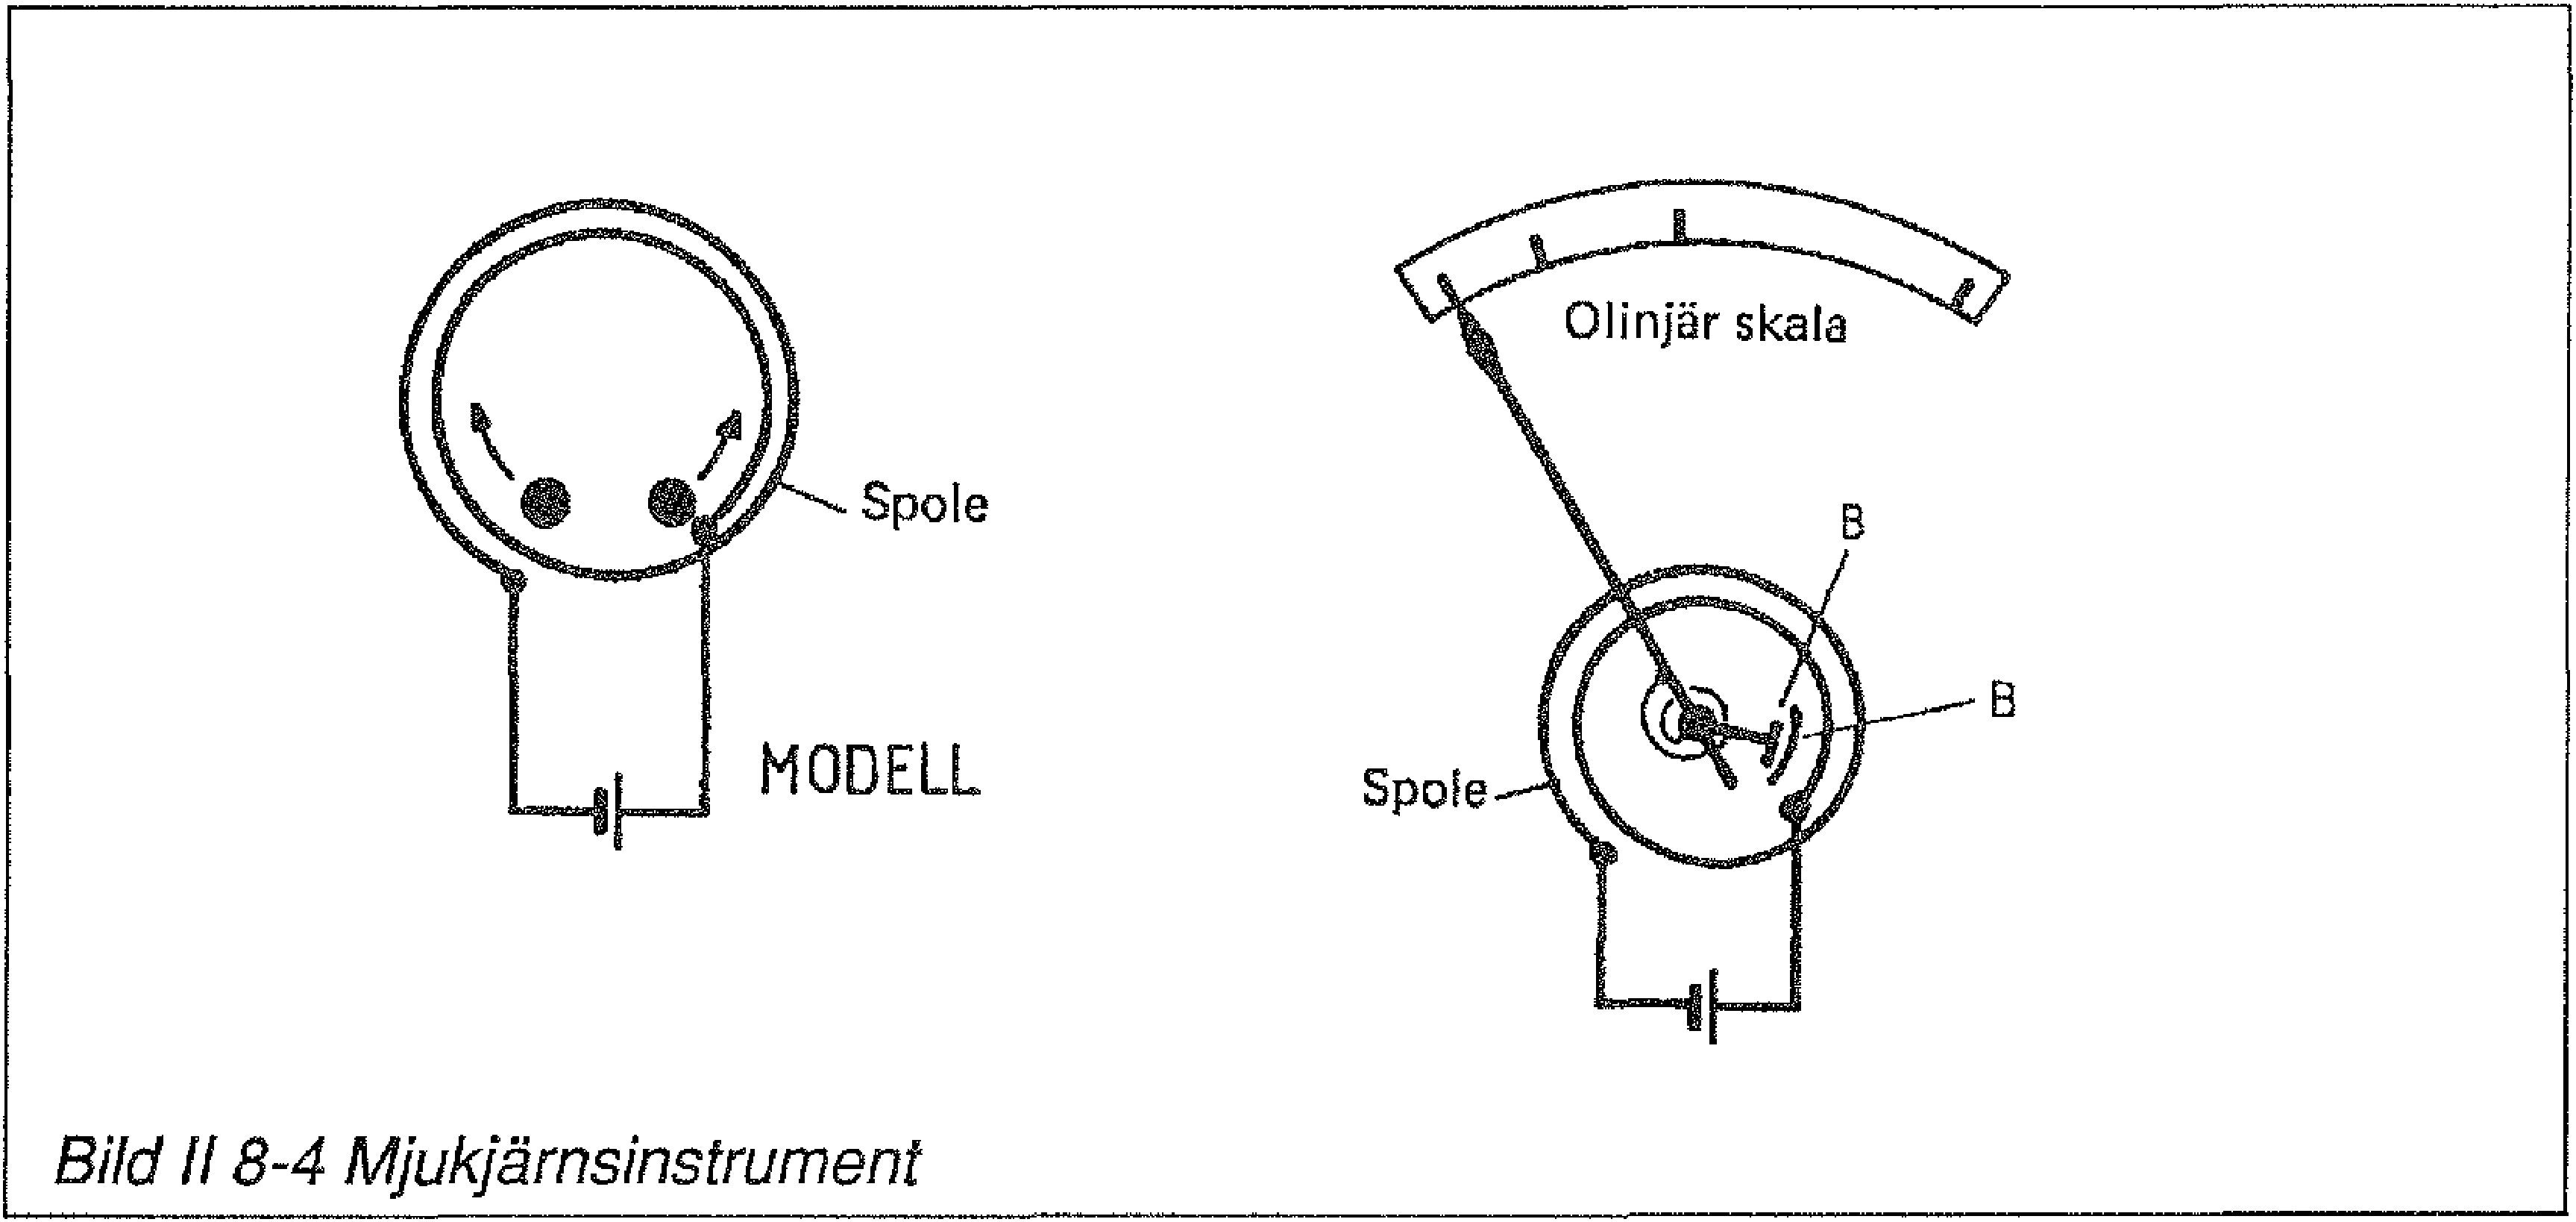
\includegraphics[width=\textwidth]{images/bild_2_8-04}
  \caption{Mjukjärnsinstrument}
  \label{fig:bildII8-4}
\end{figure}

Bild \ref{fig:bildII8-4}

Mjukjärnsinstrument kan användas för mätning av såväl lik- som
växelström. Vid växelströmsmätning kommer effektivvärdet att visas,
oavsett strömmens kurvform.

Detta instrument har en relativt dålig precision, men är användbart
för enklare ändamål. Det ersätts dock efter hand med billiga digitala
instrument.

Funktion: I ett mjukjärnsinstrument sitter två järnstycken B
placerade.  Det ena järnstycket sitter vridbart upphängt och är
försett med en returfjäder och en visare.  Det andra järnstycket
sitterfast upphängt.  Järnstyckena magnetiseras av fältet i spolen.
P.g.a. polariseringen kommer de alltid att stöta bort varandra,
oavsett strömriktningen i spolen.  Bortstötningskraften är ej
proportionell mot strömmen och skalan blir således olinjär.
\end{rev-raderas}

\begin{wrapfigure}{R}{0.5\textwidth}
  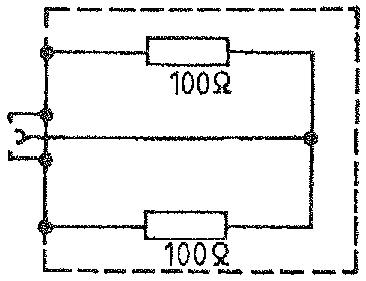
\includegraphics[width=0.5\textwidth]{images/bild_2_8-05}
  \caption{Konstlast}
  \label{fig:bildII8-5}
\end{wrapfigure}

\subsection{Konstlast}

Bild \ref{fig:bildII8-5}

En konstlast (dummy load) bör ingå i varje amatörradiostation.  Vid
mätning och inställning av t.ex. modulation och uteffekt, är det
lämpligt att belasta sändaren med dess nominella utgångsimpedans.  För
att då undvika att energi strålas ut bör en väl skärmad konstlast
användas.

I moderna amatörradiosändare med koaxialkabel utgång är
utgångsimpedansen 50~Ω. Konstlasten ska då vara en 50~Ω resistor
utan reaktiva egenskaper.  Den kan bestå av en eller flera
sammankopplade resistorer.

Sändareffekten ska kunna tas upp utan att resistansen förändras
nämnvärt. Det är viktigt att resistorerna kyls effektivt med luft
eller vätska i ett kärl med tillräckligt utrymme, även när vätskan
expanderar av värmen.  Vätskan får inte vara lättantändlig eller
miljöfarlig.  T.ex. är oljor med PCB förbjudna!

\subsection{Fältstyrkemätare}

\begin{figure}
  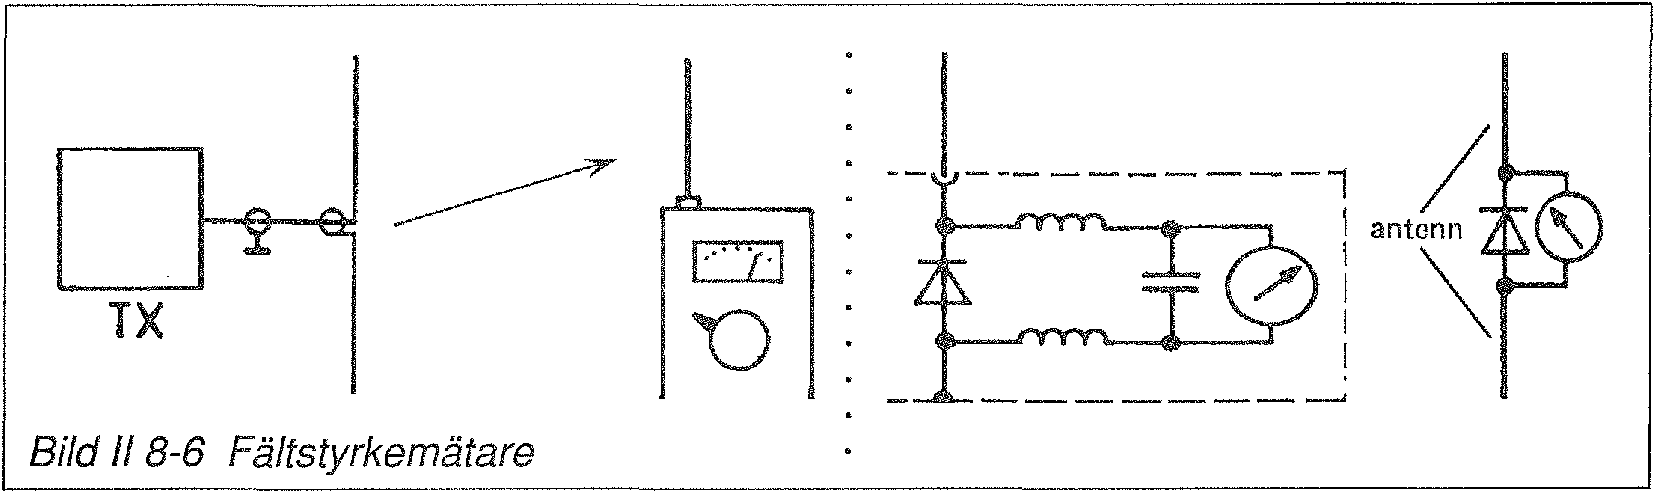
\includegraphics[width=\textwidth]{images/bild_2_8-06}
  \caption{Fältstyrkemätare}
  \label{fig:bildII8-6}
\end{figure}

Bild \ref{fig:bildII8-6}

Styrkan av elektromagnetiska fält kan bestämmas med fältstyrkemätare.

En fältstyrkemätare är en högfrekvensdetektor, vars utspänning visas
med ett instrument med skala.  Den selektiva kretsen kan bestå enbart
av den avstämda antennen, men även av ytterligare selektiva
kretsar. Instrumentet visar endast relativa värden och används
t.ex. för att bestämma strålningsegenskaperna i sändarantenner och för
antennjustering.  Mätresultatet påverkas även av utstrålning från
andra sändare inom mätarens bandbredd.  Bilden visar en sändare och en
fältstyrkemätare.  Dessutom två enkla fältstyrkemätare.

\subsection{Kalibreringsoscillator}
\textbf{
HAREC a.\ref{HAREC.a.8.2.1.4}\label{myHAREC.a.8.2.1.4}
}

\begin{wrapfigure}[12]{R}{0.5\textwidth}
  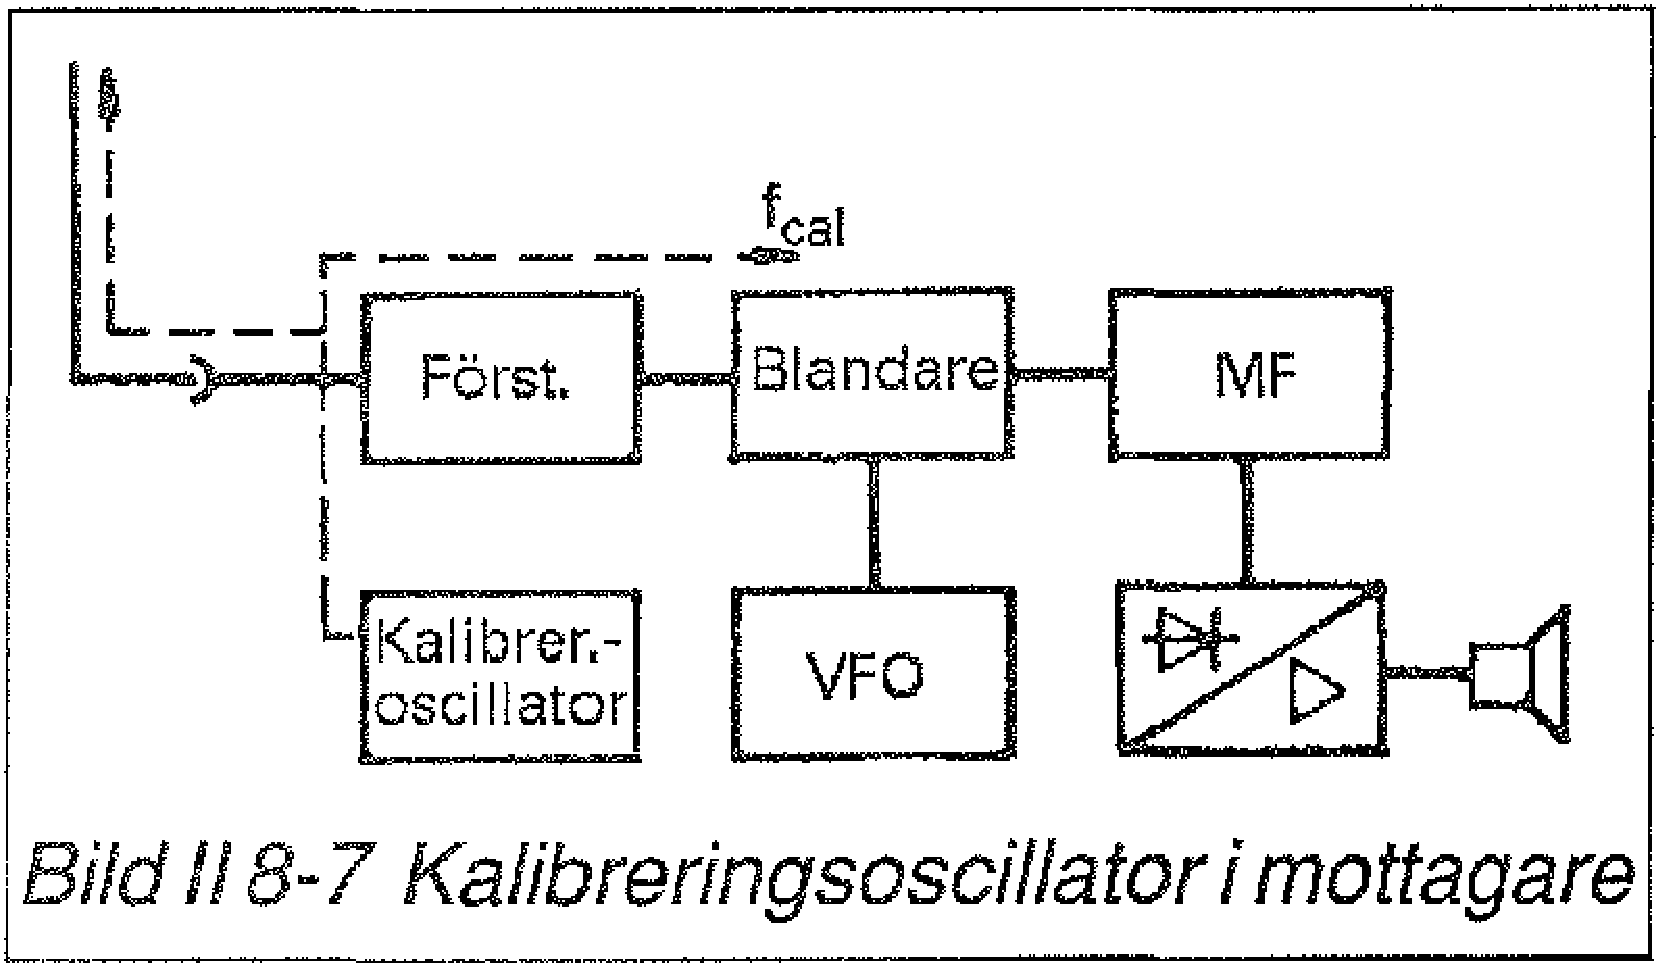
\includegraphics[width=0.5\textwidth]{images/bild_2_8-07}
  \caption{Kalibreringsoscillator i mottagare}
  \label{fig:bildII8-7}
\end{wrapfigure}

Bild \ref{fig:bildII8-7}

En kalibreringsoscillator används för att frekvenskalibrera andra
apparaters inställningsskalor.  Den är kristallstyrd och avger
särskilt precisa och frekvensstabila signaler.

Oscillatorsignalen förvrängs avsiktligt, så att det utöver
grundfrekvensen även skapas harmoniska övertoner. En oscillator med
t.ex. grundfrekvensen 25~kHz avger på så sätt även frekvenserna 50
kHz, 75~kHz, 100~kHz, 125~kHz o.s.v. Man får således en
''kalibreringsfrekvens'' för varje 25~kHz.

Detta övertonsspektrum kan sträcka flera 100~MHz upp. Man
''nollsvävar'' apparat mot närmaste kalibreringsfrekvens och kan
kalibrera t.ex. VFO-skalan.

Användningsområden:
\begin{itemize}
\item Kalibrering av mottagare och
\item Gradering av nya skalor o.s.v.
\end{itemize}

Not: Äldre trafikmottagare har VFO med LC-krets och ofta en inbyggd
kalibreringsoscillator. En kalibreringsoscillator kan i sin tur behöva
kalibreras. Det enklaste sättet är då, att jämföra frekvensen på en
känd rundradiosändare på mellanvåg med kalibreringsoscillatorn.
Dagens mottagare och sändare har syntesoscillator och då behövs
normalt ingen kalibreringsoscillator.

\subsection{Brusmätbrygga}

\begin{wrapfigure}{R}{0.5\textwidth}
  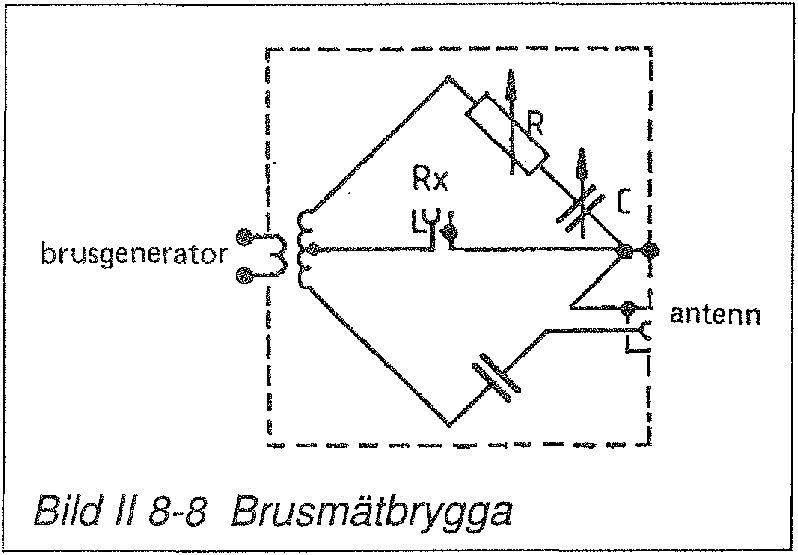
\includegraphics[width=0.5\textwidth]{images/bild_2_8-08}
  \caption{Brusmätbrygga}
  \label{fig:bildII8-8}
\end{wrapfigure}

Bild \ref{fig:bildII8-8}

Brusmätbryggan används vid mätning i antennsystem. Den består av en
brusgenerator och en Wheatstone-brygga för mätning av resistans och
reaktans.

Till bryggan ansluts en antenn som mätobjekt och en mottagare som
nollindikeringsinstrument för brussignalen. Mottagaren ställs in på
den frekvens där mätvärden önskas. Bruset hörs svagast när bryggan är
injusterad. Man kan då avläsas mätvärdena för \(R\) och \(X\). Mäter
man vid flera frekvenser, kan t.ex. ett impedansdiagram upprättas.

\subsection{Ståendevågmeter (SVF-meter)}
\textbf{
HAREC a.\ref{HAREC.a.8.2.1.3}\label{myHAREC.a.8.2.1.3}
}

\begin{figure}
  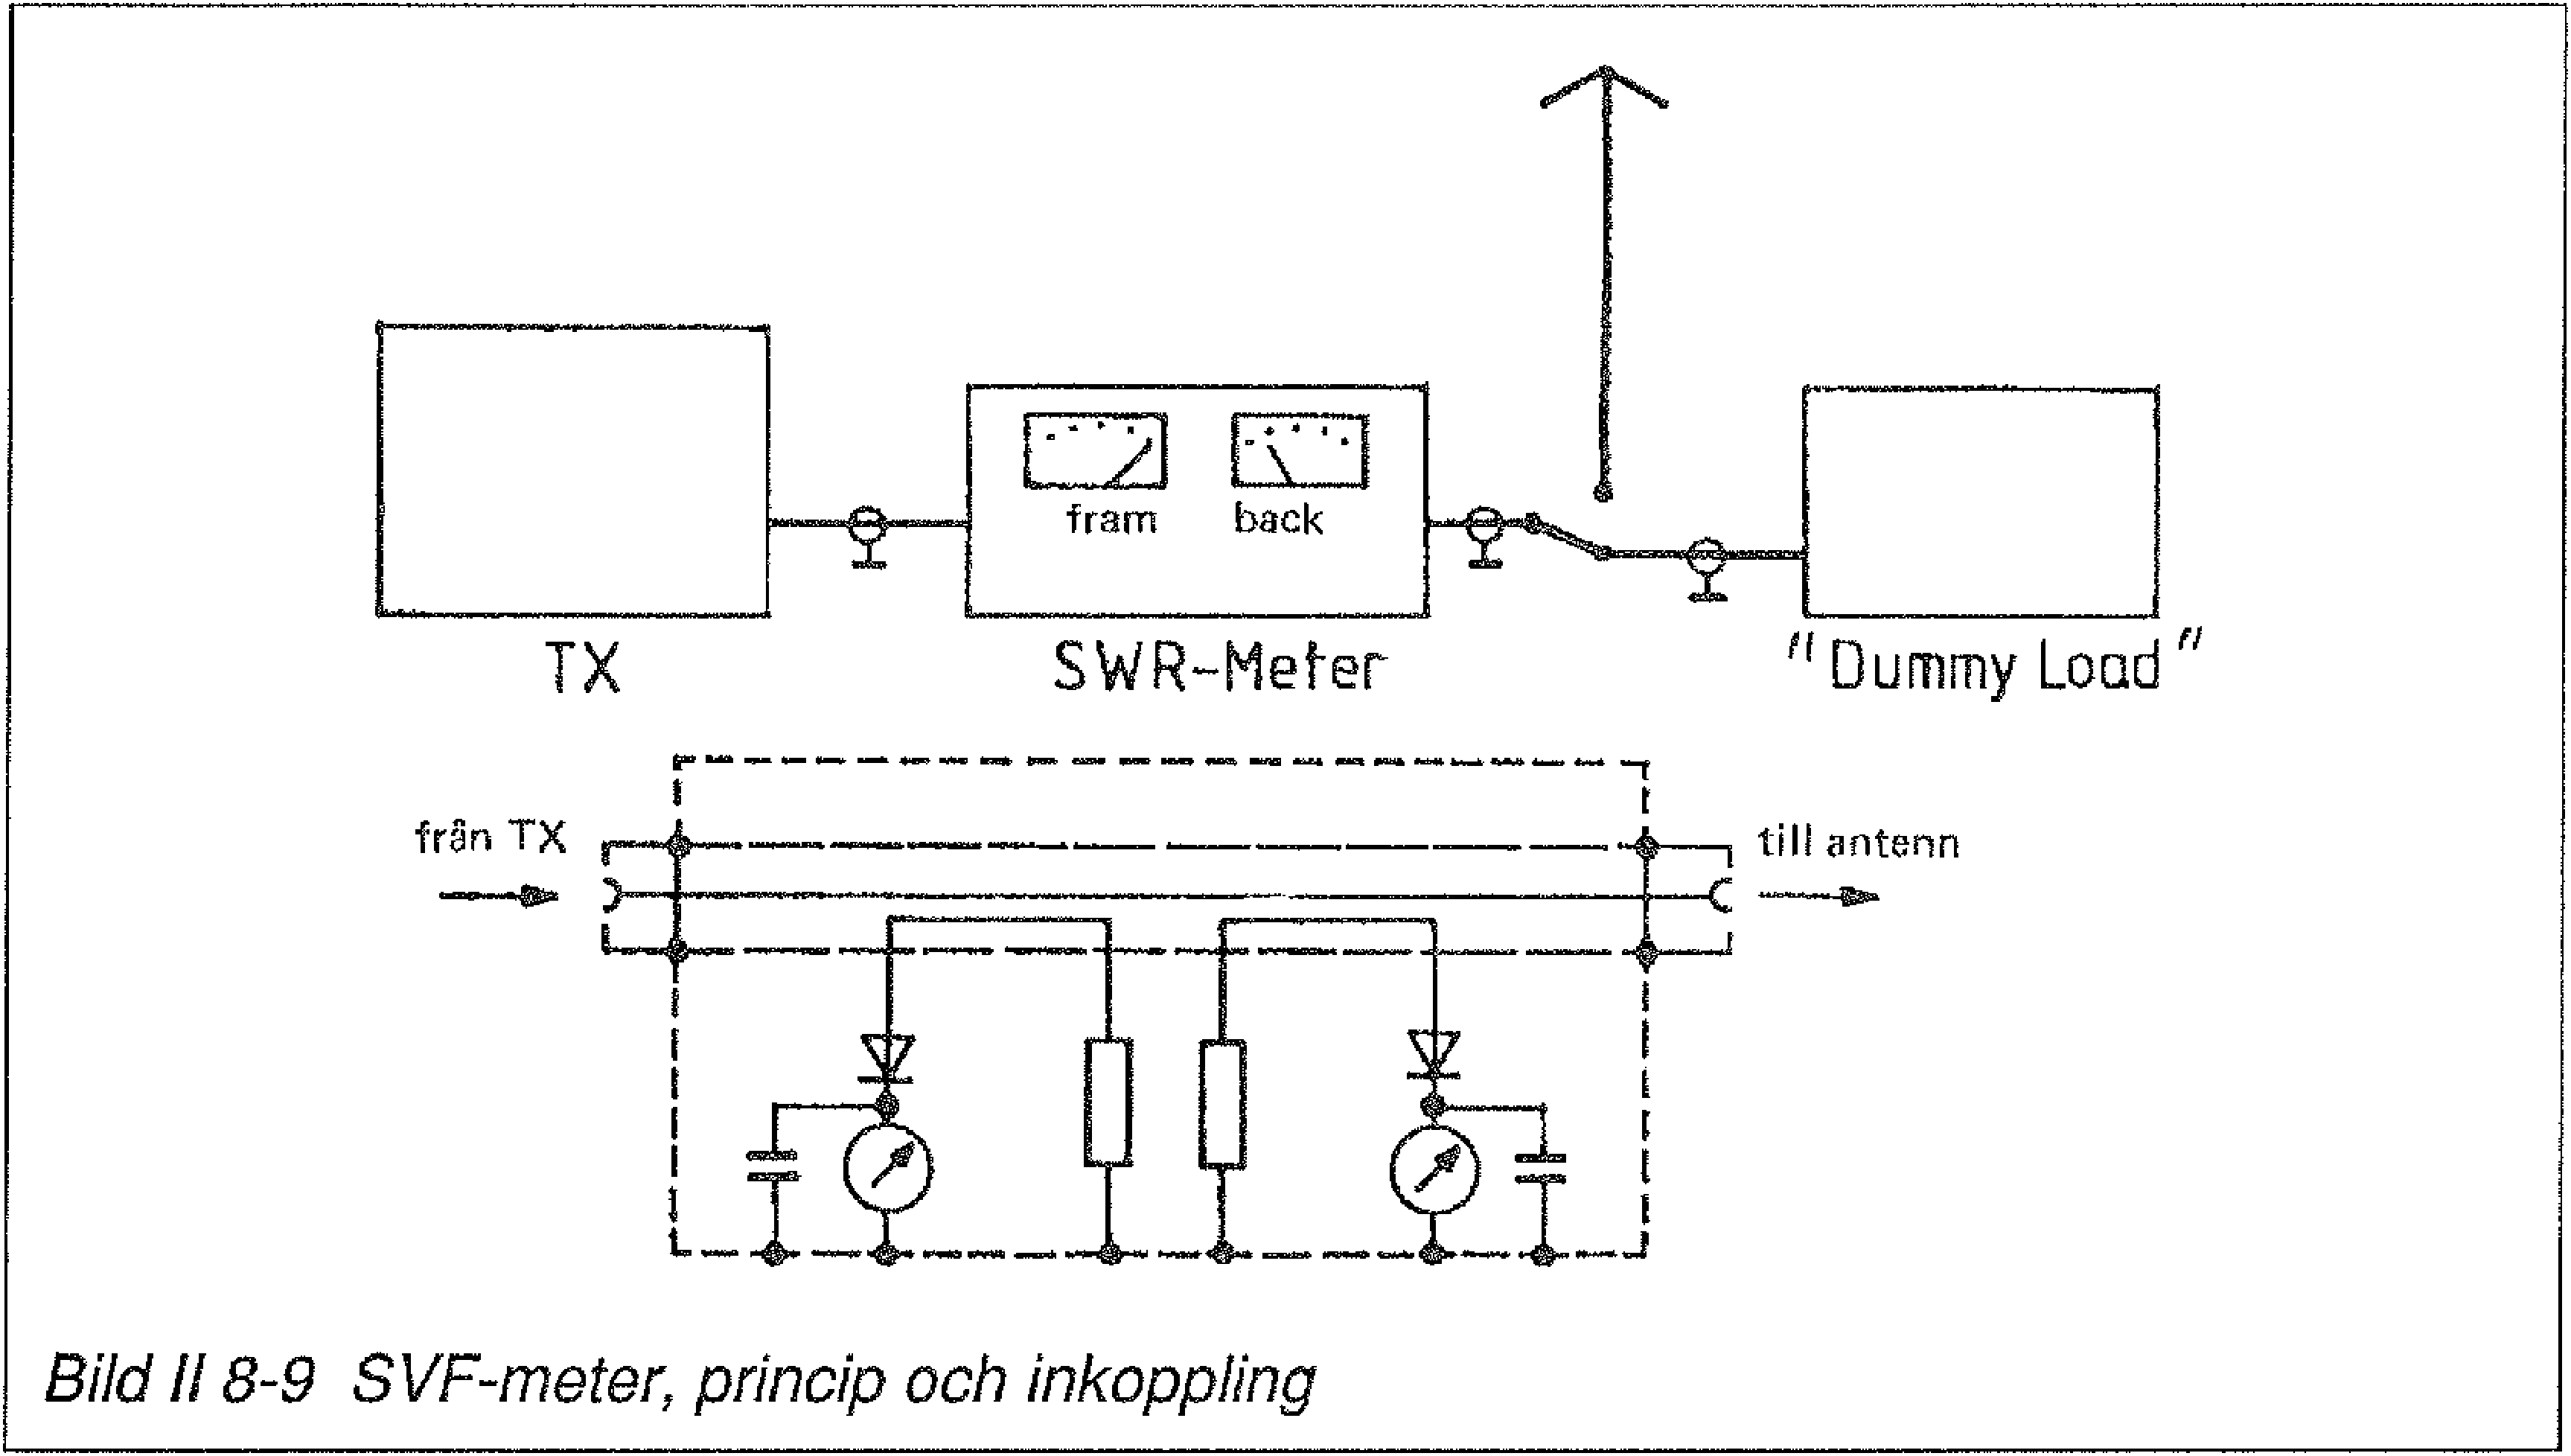
\includegraphics[width=\textwidth]{images/bild_2_8-09}
  \caption{SVF-meter, princip och inkoppling}
  \label{fig:bildII8-9}
\end{figure}

Bild \ref{fig:bildII8-9}

När en transmissionsledning eller apparat ansluts till en annan med
awikande impedans, kommer HF-energi att reflekteras i övergången.

Med ståendevåg-förhållande (SVF) eller Standing Wave Ratio (SWR)
menas förhållandet mellan den effekt som flyter framåt respektive
bakåt i en transmissionsledning.

Användningområden för SVF-meter:
\begin{itemize}
\item Mätning av framåtgående effekt.
\item Mätning av bakåtgående effekt.
\item Bestämning av SVF.
\item Bestämning av resulterande, relativ effekt.
\end{itemize}

Anmärkning: Vid bestämning av absolut effekt måste
anslutningsimpedansen vara lika i instrument och transmissionsledning.

SVF-metern är ett av de mest användbara instrumenten vid
HF-mätningar. En SVF-meter kan ha separata instrument för fram-
respektive backeffekt eller ett gemensamt.

SVF-metern kan vara ständigt inkopplad t.ex. mellan sändare och
antenn, men ska då kunna tåla effektutvecklingen. En SVF-meter kan
alstra övertoner, vilka kan medföra störningar. Orsaken är
olinjäriteten halvledardioderna i instrumentet.

\subsection{Frekvensräknare}
\textbf{
HAREC a.\ref{HAREC.a.8.2.1.5}\label{myHAREC.a.8.2.1.5}
}

\begin{wrapfigure}{R}{0.5\textwidth}
  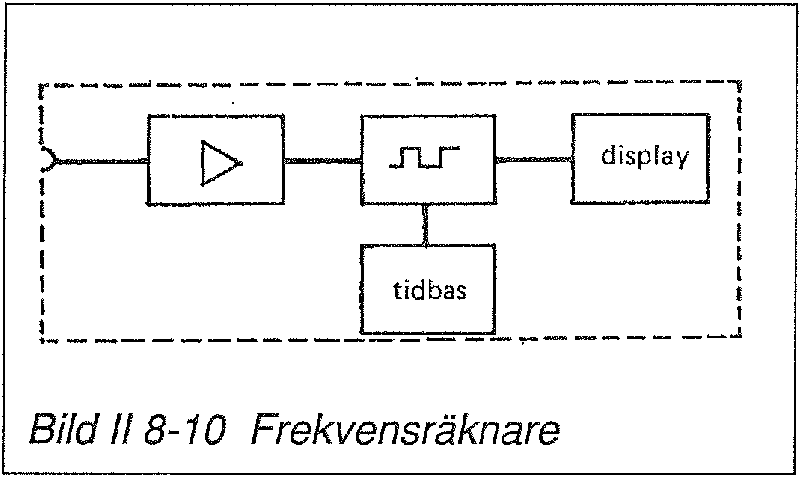
\includegraphics[width=0.5\textwidth]{images/bild_2_8-10}
  \caption{Frekvensräknare}
  \label{fig:bildII8-10}
\end{wrapfigure}

Bild \ref{fig:bildII8-10}

Frekvensräknaren, som är ett digitalt instrument, används för att
bestämma oscillatorfrekvensen i sändare, mottagare m.m.

I frekvensräknaren räknas antalet svängningar i den aktuella
inkommande signalen under en bestämd tidsenhet. Först förstärks
signalen i en analog förstärkare och omvandlas till kantvågspulser. En
elektronisk ''kontakt'', en s.k. gate, släpper därefter den behandlade
ingångssignalen vidare till en digital räknare under en viss
tid. Detta sker med stor precision och i ett periodiskt
förlopp. Antalet pulser räknas under genomsläppsperioden. Resultatet
motsvarar insignalens frekvens.

Resultatet visas som siffror i ett fönster. Noggrannheten i den
s.k. tidbasen erhålls med en kristallstyrd oscillator, vars frekvens
delas ner till önskat värde.

\begin{rev-raderas}
\subsection{Absorbtionsvågmeter}

\begin{wrapfigure}{R}{0.5\textwidth}
  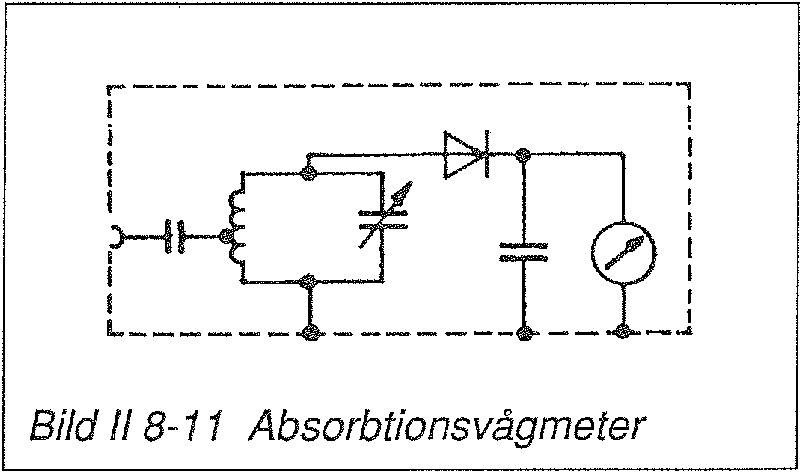
\includegraphics[width=0.5\textwidth]{images/bild_2_8-11}
  \caption{Absorbtionsvågmeter}
  \label{fig:bildII8-11}
\end{wrapfigure}

Bild \ref{fig:bildII8-11}

Absorbtionsvågmetern används för att bestämma en oscillators
arbetsfrekvens. Den består av en resonanskrets med variabel frekvens,
som kan avläsas, och ett mätinstrument som resonansindikator.

Vågmetern kopplas induktivt till den krets, vars frekvens ska
bestämmas. När frekvensen i kretsen och vågmetern stämmer överens, ger
resonansindikatorn utslag. Frekvensen avläses då på vågmeterns skala.

Anmärkning: Frekvensmätning på en passiv svängningskrets kan inte
göras med detta instrument, vilket däremot går med en
dip-meter. Principen för en absorbtionsvågmeter är annorlunda än den
för en dip-meter, men i regel kan en dip-meter också användas som
absorbtionsvågmeter.
\end{rev-raderas}

\begin{wrapfigure}{R}{0.5\textwidth}
  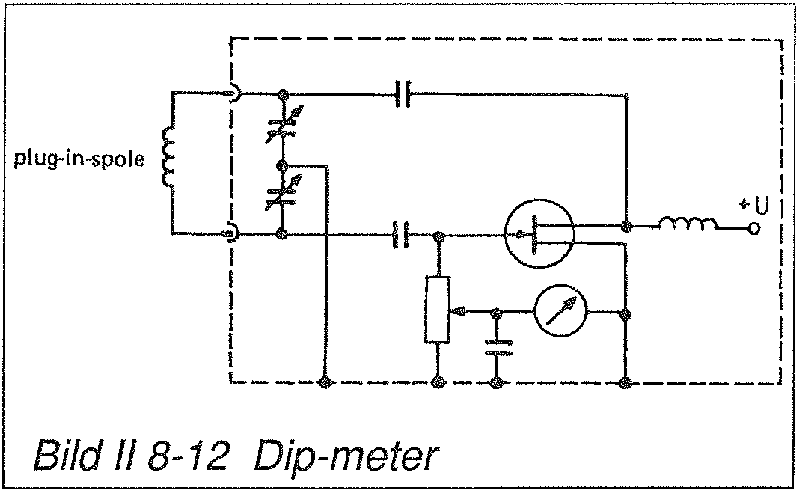
\includegraphics[width=0.5\textwidth]{images/bild_2_8-12}
  \caption{Dip-meter}
  \label{fig:bildII8-12}
%\end{wrapfigure}

%\begin{wrapfigure}{R}{0.5\textwidth}
  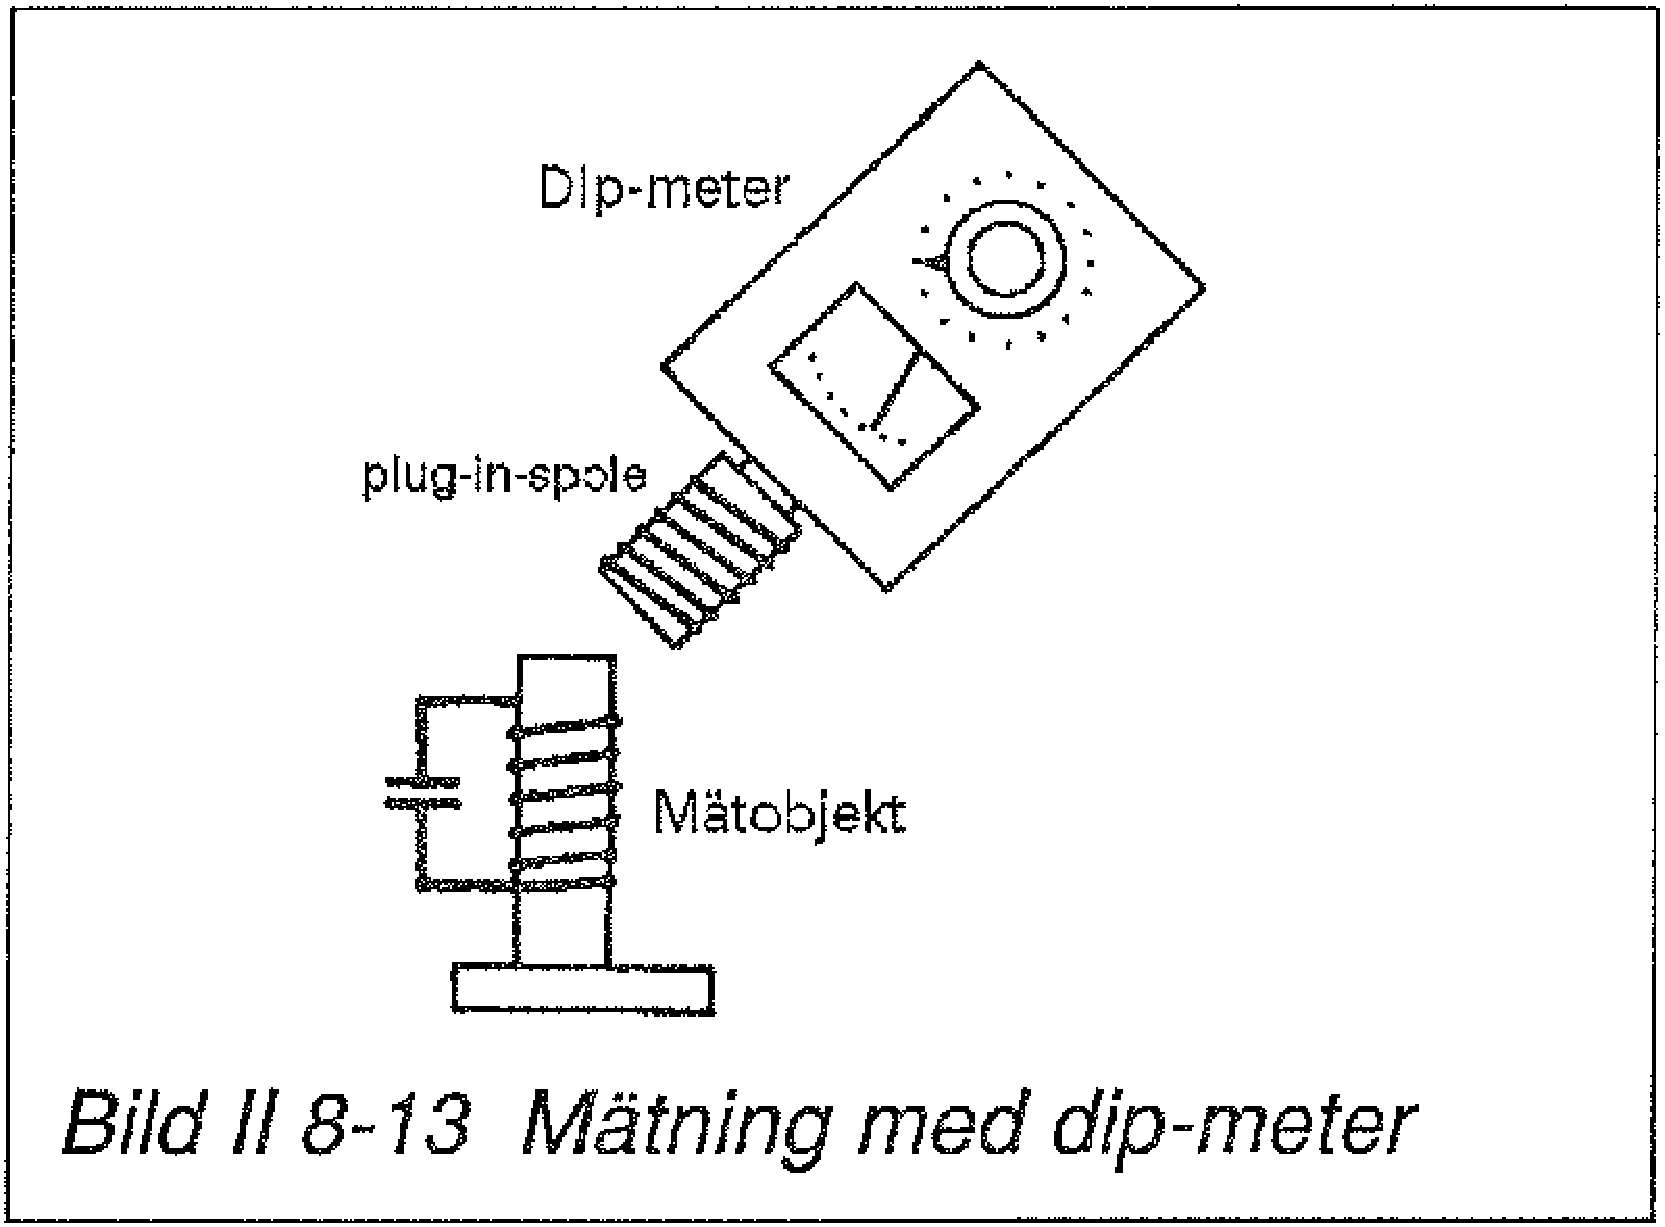
\includegraphics[width=0.5\textwidth]{images/bild_2_8-13}
  \caption{Mätning med dip-meter}
  \label{fig:bildII8-13}
\end{wrapfigure}

\subsection{Dip-meter}

Se bild \ref{fig:bildII8-12} och \ref{fig:bildII8-13}.

Dipmetern är i princip en oscillator med variabel frekvens och
utbytbara induktorer för olika frekvensområden.  Den används för att
bestämma resonansfrekvensen på passiva och aktiva svängningskretsar
samt vid bestämning av induktanser och kapacitanser.

Noggrannheten är ca 3~\%.

Funktion: Instrumentet avger alternativt reagerar för en HF-signal med
viss frekvens.  Resonansfrekvensen i dip-meterns svängningskrets är
steglöst variabel och frekvensvärdet kan avläsas på en skala.

Vid mätning av resonansfrekvensen i en passiv svängningskrets kopplas
dip-meterns induktor induktivt till kretsen. När resonansfrekvensen i
kretsen och dip-metern överensstämmer, ändras belastningen i
dip-meterns svängningskrets varvid instrumentet uppvisaren
strömminskning -- en ''dip''. Frekvensen avläses då på skalskivan.

Vid mätning på en aktiv svängningskrets, d.v.s. som drivs av någon
HF-källa, uppstår i stället en strömökning vid resonans vilket också
visas på instrumentet.

Induktansen i en svängningskrets kan bestämmas med dip-metern, om
kapacitansenär bekant. På motsvarande sätt kan en obekant kapacitans
bestämmas om induktansen i svängningskretsen är bekant.

Namnet grid-dipmeter kommer från elektronrörsepoken. Ändringar i
gallerströmmen (grid current) i ett oscillatorkopplat elektronrör
används som indikation på att en svängningskrets är i resonans. Då
minskar gallerströmmen - det blir en ''ström-dip''.  Numera används en
transistor i stället för röret och instrumentet benämns dip-meter.

\subsection{Oscilloskop}
\textbf{
HAREC a.\ref{HAREC.a.8.2.1.6}\label{myHAREC.a.8.2.1.6}
}

\begin{rev-omarbetas}
\begin{figure}
  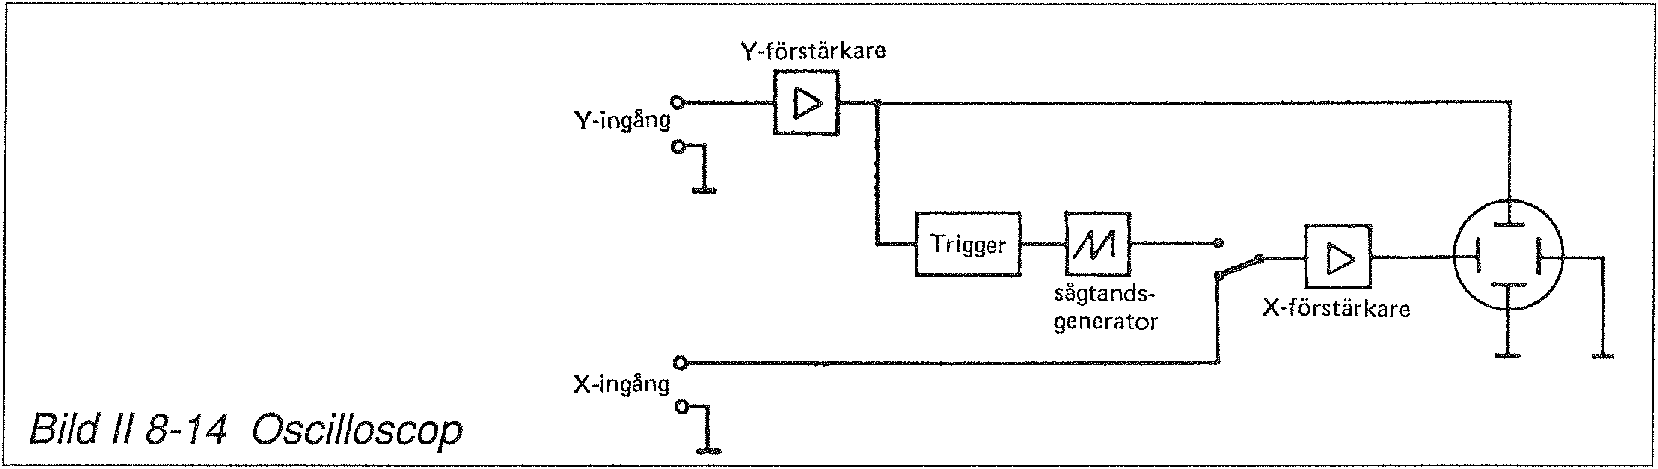
\includegraphics[width=\textwidth]{images/bild_2_8-14}
  \caption{Oscilloskop}
  \label{fig:bildII8-14}
\end{figure}

Bild \ref{fig:bildII8-14}

Oscilloskopet är ett mycket användbart instrument. Mycket snabba
förlopp kan med fördel studeras på en oscilloskopskärm.

Spänningsförlopp kan visas som funktion av tiden. Tillsammans med
andra instrument kan frekvenskaraktäristiken i filter,
modulationskvalitet o.s.v. åskådliggöras.

Oscilloskopet består av ett katodstrålerör, där styrningen av
katodstrålen sker med hjälp av X- och Y-förstärkare och en s.k.
triggerförstärkare. Den signal som ska mätas ansluts vanligen till
Y-förstärkaren medan en tidbasgenerator som alstrar en sågtandformad
signal ansluts till X-förstärkaren.  Bilden visar ett blockschema på
oscilloskop.
\end{rev-omarbetas}

\hilight{TODO: Beskriv hur man faktiskt använder ett oscilloskop och vad
man kan göra med det.}

\hilight{TODO: Beskriv digitala och PC-baserade digitala oscilloskop}

\subsection{Spektrumanalysator}

\hilight{TODO: Beskriv spektrumanalysator och vad man kan göra med den}

\subsection{Nätverksanalysator}

\hilight{TODO: Beskriv nätverksanalysator och vad man kan göra med den}
